    \documentclass[conference]{IEEEtran}
\IEEEoverridecommandlockouts
% Template version as of 6/27/2024

\usepackage{cite}
\usepackage{amsmath,amssymb,amsfonts}
\usepackage{algorithm}
\usepackage{algpseudocode}
\usepackage{graphicx}
\usepackage{textcomp}
\usepackage{xcolor}
\usepackage{booktabs}
\usepackage{url}
\usepackage{tikz}
\usetikzlibrary{arrows.meta,positioning}

% This local IEEEtran.cls copy is missing \linebreakand (used to start a new
% row of authors for a 2x2 layout). Provide the standard definition; harmless
% if a complete IEEEtran already defines it.
\makeatletter
\providecommand{\linebreakand}{%
  \end{@IEEEauthorhalign}
  \hfill\mbox{}\par
  \mbox{}\hfill\begin{@IEEEauthorhalign}}
\makeatother

\def\BibTeX{{\rm B\kern-.05em{\sc i\kern-.025em b}\kern-.08em
    T\kern-.1667em\lower.7ex\hbox{E}\kern-.125emX}}

% ---------------------------------------------------------------------------
% PLACEHOLDER MACROS
%   \ph{...}  : a numeric result still to be filled in (shown in red).
%   \fig{...} : a figure placeholder box so the draft compiles with no images.
% Search the source for "\ph{" to find every cell/number that needs a value.
% ---------------------------------------------------------------------------
\newcommand{\ph}[1]{\textcolor{red}{\textbf{#1}}}
\newcommand{\fig}[2]{%
  \fbox{\parbox[c][#1][c]{0.92\columnwidth}{\centering\itshape
    \textcolor{red}{[FIGURE PLACEHOLDER]}\\[2pt]#2}}}

\begin{document}

\title{Co-Adaptation over Allocation: KL-Guided Mixed-Precision Quantization-Aware Training}

% -------------------------------------------------------------------------
% DOUBLE-BLIND SUBMISSION: authors anonymized for review.
% Restore the real author block (below, commented out) for the camera-ready.
% -------------------------------------------------------------------------
\author{}


% --- CAMERA-READY AUTHOR BLOCK (uncomment for the final version) ---
% \author{%
% \IEEEauthorblockN{Shreya Mandekar}
% \IEEEauthorblockA{\textit{Dept. of CSE} \\
% \textit{MIT World Peace University}\\
% Pune, India \\
% mandekarofficial@gmail.com}
% \and
% \IEEEauthorblockN{Jayraj K. Ladkat}
% \IEEEauthorblockA{\textit{Dept. of CSE} \\
% \textit{MIT World Peace University}\\
% Pune, India \\
% jayrajkladkat@gmail.com}
% \linebreakand
% \IEEEauthorblockN{Madhura Phatak}
% \IEEEauthorblockA{\textit{Dept. of CSE} \\
% \textit{MIT World Peace University}\\
% Pune, India \\
% madhura.phatak@mitwpu.edu.in}
% \and
% \IEEEauthorblockN{Bhavana Tiple}
% \IEEEauthorblockA{\textit{Dept. of CSE} \\
% \textit{MIT World Peace University}\\
% Pune, India \\
% bhavana.tiple@mitwpu.edu.in}
% }

\maketitle

\begin{abstract}
Mixed-precision quantization assigns a per-layer bit-width and is the standard
route to sub-4-bit inference, where a single uniform width is too coarse. The
common recipe is \emph{post-hoc}: measure each layer's sensitivity on a fixed
trained model, freeze the assignment, and briefly fine-tune. This is simple and
effective when the budget is generous, but the assignment is made against weights
that never see the final precision, so the model cannot \emph{co-adapt} to it. This
work asks whether moving the sensitivity signal, a per-layer marginal
Kullback--Leibler (KL) divergence between the quantized and full-precision
predictive distributions, inside the training loop helps when the budget is
tightest. The proposed controller anneals the average bit-width to a target and continually
re-allocates precision while the weights are still learning. On Mamba-130M with
WikiText, this co-adaptive allocation beats a post-hoc allocator using the \emph{same}
KL signal in the aggressive sub-4-bit regime (314 vs.\ 950 perplexity at a 3-bit
average, a budget no uniform width can reach), and the advantage transfers to a
transformer (GPT-2: 56.4 vs.\ 145.1). The gain is specific to this regime: once a
uniform width can reach the budget it is simpler and Pareto-dominates all
mixed-precision methods, so co-adaptation helps precisely where a sub-4-bit average
must be hit and uniform quantization is not an option. Realizing it also requires
co-designing the precision anneal with the learning rate, which is held through
co-adaptation rather than decayed to zero. At these tight budgets co-adaptation,
not allocation, is the operative degree of freedom.
\end{abstract}

\begin{IEEEkeywords}
quantization-aware training, mixed precision, KL divergence, co-adaptation,
sensitivity analysis, state-space models, Mamba, large language models,
model compression
\end{IEEEkeywords}

\section{Introduction}
Quantizing the weights of a language model to low bit-widths is the dominant
lever for reducing its memory footprint and inference cost \cite{survey}. Below roughly four
bits, however, a single \emph{uniform} bit-width applied to every layer becomes
too blunt: some layers tolerate aggressive compression while others are
disproportionately sensitive, so a uniform setting either wastes bits on robust
layers or destroys accuracy on fragile ones. \emph{Mixed-precision}
quantization addresses this by assigning a per-layer bit-width, turning
quantization into a constrained allocation problem: spend a fixed average
bit-budget so as to minimize the loss in model quality.

The prevailing recipe for choosing this allocation is \emph{post-hoc}. One first
trains (or takes) a high-precision model, measures a per-layer sensitivity score
on that fixed model -- via the Hessian \cite{hawq} or, most relevant here, the KL
divergence between the quantized and full-precision output distributions
\cite{kllens} -- and then assigns bit-widths greedily under the budget. A short recovery fine-tune follows. Crucially, the
sensitivity is measured against a model whose weights were never trained at the
target precision, and the assignment is frozen before fine-tuning.

This ordering is effective and inexpensive, but it leaves one degree of freedom
unused: the ability of the weights to \emph{co-adapt} to the precision they will
ultimately run at. A layer that looks fragile at full precision may become robust
if its neighbours are trained to compensate for its quantization noise -- but only
if the allocation and the weights are learned \emph{together}. Whether exploiting
this degree of freedom is worthwhile turns out to depend on the budget, as shown below.

The allocation decision is therefore moved inside training. The KL
sensitivity signal of \cite{kllens} is retained, but computed \emph{during training}, against the
current (partially quantized) weights, and used to drive a closed-loop
controller. The controller (i) anneals the network's average bit-width from full
precision down to a target budget over the course of training, (ii) at each step
greedily lowers the precision of the layer whose marginal KL cost per bit is
smallest, and (iii) raises (``recovers'') the precision of any layer whose marginal
KL has spiked. Because every precision change happens while the optimizer is
still running, the surviving high-precision layers learn to absorb the error
introduced by the compressed ones.

\noindent\textbf{Contributions.}
\begin{itemize}
\item Mixed-precision allocation is recast as a co-adaptation problem and
instantiated as a budgeted, KL-guided precision controller for
quantization-aware training (Section~\ref{sec:method}).
\item Co-adaptive allocation is shown to beat a faithful post-hoc KL allocator at
matched average bit-width on Mamba-130M, with the advantage concentrated in the
sub-4-bit regime (B3/B4) and transferring from this SSM to a transformer (GPT-2);
the boundary beyond which the method ceases to help is reported (above $\approx$4-bit
average, post-hoc is competitive or better) (Section~\ref{sec:results}). The controller's converged
allocation is further shown to be uncorrelated with the post-hoc one (Cohen's \(\kappa\!\approx\!0\)),
locating the benefit in co-adaptation rather than in the bit assignment itself.
\item A coupling unique to the co-adaptive setting is identified, and the schedule is co-designed
around it: because a learning-rate schedule that decays to zero (standard for the
baselines) would land the largest precision drops when the model can no longer
adapt, the learning rate is held through the co-adaptation phase and
precision is annealed gradually -- found necessary for stable convergence in the
aggressive sub-4-bit regime (Sections~\ref{ssc:schedule} and \ref{ssc:stability}).
\end{itemize}

\section{Background and Related Work}
\subsection{Quantization-aware training}
Quantization-aware training (QAT) simulates low-precision arithmetic in the
forward pass while keeping a full-precision copy of the weights for the backward
pass. The non-differentiable rounding operator is handled with the
straight-through estimator (STE) \cite{ste}, which passes gradients through the
quantizer unchanged. QAT consistently outperforms post-training quantization at
low bit-widths because the weights learn to be robust to the quantization noise
\cite{jacob,lsq}.

\subsection{Mixed-precision allocation}
Given a per-layer sensitivity score, mixed-precision methods allocate bit-widths
under an average-bit budget. HAWQ \cite{hawq} and its successors
\cite{hawqv2,hawqv3} rank layers by Hessian curvature, and HAQ \cite{haq} searches
the allocation with reinforcement learning; post-training methods such as GPTQ
\cite{gptq} instead minimize layer-wise reconstruction error at a fixed width. The
KL-based allocator used here as a baseline
(referred to as the post-hoc KL baseline \cite{kllens})
scores each layer by the increase in KL divergence between the quantized and
full-precision predictive distributions when that layer is dropped to the next
lower bit-width, and assigns greedily. All of these operate on a \emph{fixed} model
and freeze the allocation before any (optional) recovery fine-tune.

A separate line of work \emph{learns} bit-widths during training by introducing
extra differentiable architecture or gating parameters: differentiable
architecture search over precisions \cite{dnas,edmips}, learned bit-width
parametrizations \cite{dq}, and fractional bit-widths \cite{fracbits}. The method
presented here acts during training in the same temporal sense, but differs in both mechanism and intent: it
adds \emph{no} learnable allocation parameters and instead drives a closed-loop
controller from a forward-only, gradient-free KL signal -- the very signal used by
the post-hoc baseline. This attributes any gain to \emph{co-adaptation}
itself rather than to a richer, separately optimized search space.

Closest in spirit are switchable-precision networks -- any-precision
\cite{anyprec}, AdaBits \cite{adabits}, and Bit-Mixer \cite{bitmixer} -- which
train a single network whose weights tolerate \emph{many} bit-widths selected at
runtime. The present approach instead co-adapts the weights to \emph{one} allocation chosen under a
budget. Finally, the sensitivity signal used here -- the KL divergence to a full-precision
teacher -- is the same quantity minimized in self-distillation \cite{distill,polino};
here it serves only to guide allocation, not as a training loss.

\subsection{State-space models}
Evaluation is primarily on Mamba \cite{mamba}, a selective state-space model whose
mixer is built from projection linear layers (the closely related Mamba-2
\cite{mamba2} shares this structure), with GPT-2 \cite{gpt2} used to test transfer to
a non-SSM (attention) architecture. Only the projection linear layers
(the bulk of the parameters) are quantized, leaving convolutions, the selective scan, and
normalization in full precision, matching the protocol of the post-hoc KL baseline.

\section{Method}
\label{sec:method}
The method computes the post-hoc KL sensitivity signal \emph{during} training and
lets a budgeted controller re-allocate precision while the weights are still
learning. Fig.~\ref{fig:method} contrasts this timeline with the post-hoc baseline,
which scores and freezes the bit-width on a trained model before a short fine-tune.

\begin{figure}[t]
\centering
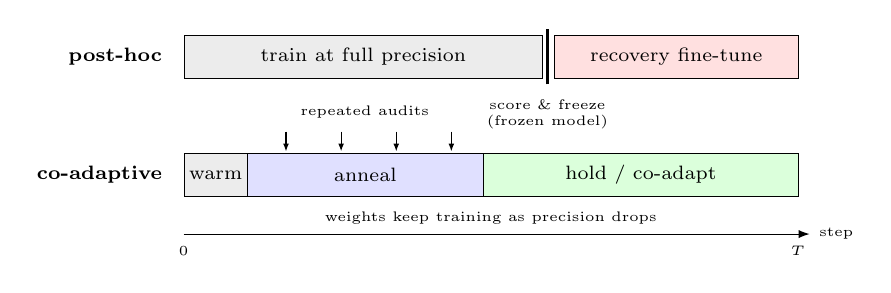
\begin{tikzpicture}[font=\scriptsize,
  bar/.style={anchor=west, minimum height=0.55cm, draw, align=center, inner sep=1pt}]

% ---------- post-hoc row (top) ----------
\node[bar, minimum width=4.55cm, fill=gray!15] (pt) at (0,1.5) {train at full precision};
\node[bar, minimum width=3.10cm, fill=red!12]  (pr) at (4.70,1.5) {recovery fine-tune};
\node[anchor=east, font=\scriptsize\bfseries] at (-0.15,1.5) {post-hoc};
\draw[very thick] (4.62,1.15) -- (4.62,1.85);
\node[font=\tiny, anchor=north, align=center] at (4.62,1.08)
  {score \&\ freeze\\(frozen model)};

% ---------- co-adaptive row (bottom) ----------
\node[bar, minimum width=0.80cm, fill=gray!15]  (ow) at (0,0.0) {warm};
\node[bar, minimum width=3.00cm, fill=blue!12]  (oa) at (0.80,0.0) {anneal};
\node[bar, minimum width=4.00cm, fill=green!14] (oh) at (3.80,0.0) {hold / co-adapt};
\node[anchor=east, font=\scriptsize\bfseries] at (-0.15,0.0) {co-adaptive};
\foreach \x in {1.3,2.0,2.7,3.4}{
  \draw[-{Latex[length=1mm]}] (\x,0.55) -- (\x,0.30);}
\node[font=\tiny, anchor=south] at (2.30,0.60) {repeated audits};
\node[font=\tiny, anchor=north, align=center] at (3.90,-0.34)
  {weights keep training as precision drops};

% ---------- shared step axis ----------
\draw[-{Latex[length=1.4mm]}] (0,-0.75) -- (7.95,-0.75)
  node[anchor=west, font=\tiny] {step};
\node[font=\tiny, anchor=north] at (0,-0.78) {0};
\node[font=\tiny, anchor=north] at (7.80,-0.78) {$T$};
\end{tikzpicture}
\caption{Post-hoc vs.\ co-adaptive allocation on a shared training timeline.}
\label{fig:method}
\end{figure}

\subsection{Quantization setup}
Weights are quantized to a small discrete bit set \(\mathcal{B}=\{2,4,8\}\) with
symmetric \emph{per-output-channel} STE fake quantization. Mixed precision lives
entirely on the weights: activations use a fixed dynamic per-token 8-bit scheme
for every method, matching the post-hoc KL baseline. Each quantizable layer \(l\)
holds a current weight bit-width
\(b_l \in \mathcal{B}\). A configuration is summarized by its parameter-weighted
average bit-width,
\begin{equation}
\bar{b} \;=\; \frac{\sum_l n_l\, b_l}{\sum_l n_l},
\label{eq:avgbits}
\end{equation}
where \(n_l\) is the number of weights in layer \(l\). A budget target
\(B^\star\) is a value of \(\bar{b}\). Because \(\mathcal{B}\) is coarse, a 3-bit
average is reachable \emph{only} by mixed precision (there is no 3 in
\(\mathcal{B}\)), which is precisely the regime that motivates the approach.

\subsection{Marginal-KL sensitivity audit}
Let \(p^{\text{FP}}\) be the next-token distribution of the full-precision model
and \(p^{\theta}\) that of the current (partially quantized) model on a small
fixed calibration batch. Each layer's sensitivity is measured by a
\emph{forward-only} audit using the divergence \(D_{\mathrm{KL}}(p^{\theta}\,\|\,
p^{\text{FP}})\), the \emph{student-to-teacher} (mode-seeking) direction, matching
the post-hoc KL baseline \cite{kllens} so that any difference between the two
methods is attributable to \emph{when} the signal is applied rather than to a
different sensitivity measure. A KL divergence to the full-precision teacher is a
principled proxy for the perplexity gap: treating the full-precision model as the
reference distribution, the quantization-induced increase in next-token
cross-entropy is \(D_{\mathrm{KL}}(p^{\text{FP}}\,\|\,p^{\theta})\), so
\(\mathrm{PPL}(p^{\theta}) = \mathrm{PPL}(p^{\text{FP}})\exp
D_{\mathrm{KL}}(p^{\text{FP}}\,\|\,p^{\theta})\). The student-to-teacher divergence
used in the audit penalizes the quantized model for placing probability mass where
the teacher does not, and is retained here for fidelity to the baseline allocator. For layer \(l\), let \(b_l^- =
\max\{b\in\mathcal{B}: b<b_l\}\) and \(b_l^+ = \min\{b\in\mathcal{B}: b>b_l\}\).
Temporarily setting layer \(l\) to \(b_l^-\) (resp.\ \(b_l^+\)) and re-measuring
the KL divergence to the full-precision teacher gives the marginal cost of
dropping and the marginal gain of raising:
\begin{align}
\Delta^{\downarrow}_l &= D_{\mathrm{KL}}\!\big(p^{\theta,\,l\to b_l^-} \,\|\, p^{\text{FP}}\big) - D_{\mathrm{KL}}\!\big(p^{\theta} \,\|\, p^{\text{FP}}\big), \label{eq:down}\\
\Delta^{\uparrow}_l   &= D_{\mathrm{KL}}\!\big(p^{\theta} \,\|\, p^{\text{FP}}\big) - D_{\mathrm{KL}}\!\big(p^{\theta,\,l\to b_l^+} \,\|\, p^{\text{FP}}\big). \label{eq:up}
\end{align}
Critically, the audit measures KL at the layer's \emph{actual} current precision
rather than re-fitting an idealized scale, so that accumulated staleness is
visible to the controller. The audit is forward-only and uses a small
calibration batch, so its cost is a small multiple of one forward pass.

\subsection{Budgeted precision controller}
Training proceeds in three phases over the total step budget, parameterized by
fractions \(f_{\text{warm}}\) and \(f_{\text{hold}}\):
\begin{itemize}
\item \textbf{Warmup} \([0, f_{\text{warm}})\): all layers at 8-bit; gather
statistics; no precision changes.
\item \textbf{Anneal} \([f_{\text{warm}}, f_{\text{hold}})\): the target average
bit-width descends linearly from 8 to \(B^\star\); the controller drops layers to
keep pace.
\item \textbf{Hold / co-adapt} \([f_{\text{hold}}, 1]\): target pinned at
\(B^\star\); the weights co-adapt to the final precision.
\end{itemize}
Recovery (precision raises) runs at every audit after warmup, in both the anneal
and hold phases.
At each audit (every \(T_{\text{anneal}}\) steps during the anneal,
\(T_{\text{hold}}\) steps thereafter) the controller first raises (``recovers'')
any layer whose \(\Delta^{\uparrow}_l\) exceeds the \(P\)-th percentile of the
audit's \(\Delta^{\uparrow}\) values, then drops the layer with the smallest
\emph{cost per bit}, \(\Delta^{\downarrow}_l / (b_l - b_l^-)\), repeating the drop
until \(\bar{b}\) meets the current target; recovering before dropping keeps the
configuration at or below the budget. To keep pace with the descending target,
drops ignore the per-layer cooldown during the anneal; in the hold phase the
cooldown gates both drops and raises, and a cap on the number of raises per layer
prevents thrashing and guarantees termination. The settings are \(f_{\text{warm}}
=0.10\), \(f_{\text{hold}}=0.50\), \(P=90\), a raise cap of 3 per layer, and a
cooldown of 500 steps. Algorithm~\ref{alg:ctrl} summarizes one audit.

\begin{algorithm}[t]
\caption{Controller update at audit step \(t\)}
\label{alg:ctrl}
\begin{algorithmic}[1]
\State compute audit \(\{\Delta^{\downarrow}_l, \Delta^{\uparrow}_l\}\) on calibration batch
\State \(\tau \gets \text{target\_avg\_bits}(t)\) \Comment{linear anneal 8\(\to B^\star\)}
\For{each layer \(l\) with \(\Delta^{\uparrow}_l > \text{percentile}_P\)} \Comment{recover}
  \If{\(l\) not in cooldown \textbf{and} raise-count\(_l <\) RAISE\_CAP}
     \State raise \(b_l \to b_l^+\); start cooldown on \(l\)
  \EndIf
\EndFor
\While{\(\bar{b} > \tau\)} \Comment{drop to meet budget}
  \State \(l^\star \gets \arg\min_l \Delta^{\downarrow}_l / (b_l - b_l^-)\)
  \State drop \(b_{l^\star} \to b_{l^\star}^-\); start cooldown on \(l^\star\)
\EndWhile
\end{algorithmic}
\end{algorithm}

\subsection{Schedule co-design}
\label{ssc:schedule}
The co-adaptive setting introduces a coupling absent from post-hoc methods: a
precision drop is a discrete shock to the loss that the optimizer must recover
from \emph{within} the remaining training budget. Two design choices make this
possible.

\noindent\textbf{Gradual anneal.}
If audits are infrequent relative to the speed of the descending target, the
controller dumps many simultaneous drops at each audit (e.g.\ an
\(8\!\to\!5\)-bit average step in one window). A single large shock is far harder
to absorb than several small ones. Audits are therefore run \emph{more frequently
during the anneal} so the \(8\to B^\star\) descent is spread over many small
drops.

\noindent\textbf{Learning rate held through co-adaptation.}
A cosine schedule decaying to zero -- standard for the uniform and post-hoc
baselines -- places the largest precision drops at a point where the learning
rate, and thus the capacity to adapt, is nearly zero. For the co-adaptive method the
learning rate is instead held at its peak through the anneal and co-adaptation
phases and decayed only over the final tail of training; Section~\ref{ssc:stability}
discusses why this matters most in the aggressive sub-4-bit regime.

\section{Experimental Setup}
\label{sec:setup}
\noindent\textbf{Models.} Mamba-130M is the primary model (3 seeds); GPT-2 (124M)
is used to test transfer to a non-SSM (attention) architecture (3 seeds). The
projection linears are wrapped with fake quantization: 96 layers in Mamba-130M
(\texttt{in\_proj}, \texttt{x\_proj}, \texttt{dt\_proj}, \texttt{out\_proj} across
24 blocks) and 48 in GPT-2.

\noindent\textbf{Data and metric.} Models are trained on WikiText-103 and
evaluated by perplexity on WikiText-2 \cite{wikitext}, matching the post-hoc KL
baseline's protocol \cite{kllens}. Optimization uses AdamW \cite{adamw}.

\noindent\textbf{Baselines.}
(i) \emph{uniform}: a single bit-width for all layers, \(b\in\{2,4,8\}\);
(ii) \emph{post-hoc-base}: the 8-bit base model;
(iii) \emph{post-hoc}: the KL-based allocator \cite{kllens}, assign bit-widths
greedily on the frozen base model, then a short recovery fine-tune (1000 steps);
(iv) \emph{co-adaptive}: the proposed controller.

\noindent\textbf{Budgets.} Average-bit targets are swept over \(B^\star \in
\{3,4,5,6\}\). A 3-bit average is reachable only by mixed precision (there is no
3 in \(\mathcal{B}\)), and uniform 2-bit collapses, so the sub-4-bit regime is
precisely where mixed precision is forced; a 4-bit average is the head-to-head
against uniform 4-bit.

\noindent\textbf{Protocol.} All methods share the same model, data, sequence
length, and batch size. The uniform and co-adaptive methods train for 1500 steps
from initialization; the post-hoc allocator instead starts from a shared 1500-step
8-bit base and then runs a 1000-step recovery fine-tune, so it consumes \emph{more}
total optimization than the co-adaptive method, not less. The sub-4-bit co-adaptive
advantage is therefore obtained at no compute premium over the baselines. Because
the bit set is coarse, exact equality of \(\bar{b}\) across
methods is impossible; comparison is therefore made on the Pareto curve at the
\emph{achieved} average bit-width as well as by nominal budget.
Training runs for 1500 steps on sequences of length 512 with batch size 8 and
AdamW at a peak learning rate of $5{\times}10^{-5}$. The uniform and post-hoc
baselines use a cosine schedule decayed to zero; the co-adaptive method uses the held
schedule of Section~\ref{ssc:schedule}. The co-adaptive controller audits every
$T_{\text{anneal}}=100$ steps during the anneal phase and every
$T_{\text{hold}}=250$ steps during the hold phase, using 8 calibration sequences of
length 256; the complete hyperparameter list is in Table~\ref{tab:hparams}. All
runs were performed on a system with two NVIDIA RTX A4500 GPUs;
Mamba uses a pure-PyTorch selective scan (no fused CUDA kernel).

\section{Results}
\label{sec:results}

\subsection{Co-adaptive vs.\ post-hoc at matched budget}
Table~\ref{tab:main} reports perplexity by method and budget on Mamba-130M.
Co-adaptive beats post-hoc at B3 (314 vs.\ 950, all three seeds individually). At
B4 co-adaptive wins on the mean (99.6 vs.\ 169) and is far more stable (sd 23 vs.\
209), but this mean gap is created entirely by one post-hoc seed that diverged to
410: on the other two B4 seeds post-hoc is in fact lower (42.8, 54.4 vs.\ 74.9,
121.2). The B4 result is therefore best read as co-adaptive being more
\emph{reliable}, not as a uniform win. Above B4 the ordering is clear: post-hoc
wins at B5 (30.0 vs.\ 51.1) and B6 (19.8 vs.\ 34.7). Uniform-4-bit (19.8 PPL) Pareto-dominates all mixed-precision
methods at $\geq$4 bits. Notably, both B3 models remain far from the
full-precision baseline (17.8 PPL): at a 3-bit average the comparison is between
two heavily degraded models, so the B3 result should be read as which allocator
degrades \emph{less}, not as a deployable operating point. The paired difference
$\Delta\text{ppl} = \text{ppl}_{\text{post-hoc}} - \text{ppl}_{\text{co-adaptive}}$
(positive favours co-adaptive) has mean 352.8 across 6 matched (seed $\times$
sub-4-bit budget) pairs, with a bootstrap 95\% CI of $[79, 635]$ (10{,}000
resamples). The interval excludes zero, but it is computed over only six pairs and
is sensitive to the single diverged post-hoc seed at B4, so it should be read as
suggestive rather than conclusive; a Wilcoxon signed-rank test on the same pairs
is not significant ($p=0.156$). The B3 result does not depend on this test: co-adaptive
beats post-hoc at every individual B3 seed (251, 183, 509 vs.\ 563, 1015, 1273);
Table~\ref{tab:perseed} lists all per-seed values.

\begin{table}[t]
\caption{Mamba-130M perplexity by method and budget (mean$\pm$sd, 3 seeds; lower is
better, \textbf{bold} = best). Bits are achieved averages; $\dagger$ one diverged seed.}
\label{tab:main}
\begin{center}
\begin{tabular}{llcc}
\toprule
\textbf{Budget} & \textbf{Method} & \textbf{avg.\ bits} & \textbf{PPL (mean$\pm$sd)} \\
\midrule
B3 & post-hoc           & 2.95 & 950 $\pm$ 360 \\
B3 & \textbf{co-adaptive}    & 2.96 & \textbf{314 $\pm$ 172} \\
\midrule
B4 & \textbf{uniform-4} & 4.00 & \textbf{19.8 $\pm$ 0.0} \\
B4 & post-hoc           & 3.98 & 169 $\pm$ 209$^\dagger$ \\
B4 & co-adaptive             & 3.98 & 99.6 $\pm$ 23.3 \\
\midrule
B5 & \textbf{post-hoc}  & 4.96 & \textbf{30.0 $\pm$ 7.3} \\
B5 & co-adaptive             & 4.98 & 51.1 $\pm$ 8.3 \\
\midrule
B6 & \textbf{post-hoc}  & 5.93 & \textbf{19.8 $\pm$ 0.6} \\
B6 & co-adaptive             & 5.97 & 34.7 $\pm$ 3.3 \\
\midrule
--  & uniform-2          & 2.00 & 702 $\pm$ 1 \\
--  & uniform-8 / base-8 & 8.00 & 17.8 $\pm$ 0.0 \\
\bottomrule
\end{tabular}
\end{center}
\end{table}

\subsection{The Pareto frontier and the regime story}
Figure~\ref{fig:pareto} plots perplexity against achieved average bit-width for
all three method families. Two regimes emerge. Below four bits, mixed precision
is the only way to hit the budget, and co-adaptive dominates post-hoc. At and above
four bits, uniform quantization Pareto-dominates every mixed-precision option:
when a uniform bit-width can reach the budget, the simpler method wins. The
practical decision rule is therefore to use co-adaptive mixed precision only in the
sub-4-bit regime.

\begin{figure}[t]
\centering
\includegraphics[width=0.95\columnwidth]{fig_pareto.pdf}
\caption{Perplexity vs.\ achieved average weight-bits on Mamba-130M (3-seed mean,
log scale).}
\label{fig:pareto}
\end{figure}

\subsection{Evidence of co-adaptation}
Figure~\ref{fig:traj} shows training trajectories (loss and average bit-width vs.\
step). For the co-adaptive method the loss falls again in the second half of training,
\emph{after} the precision has reached the budget -- direct evidence that the
surviving weights co-adapt to the final precision. Quantitatively, the co-adaptive
training loss drops a further $11\%$ at B3 and $19\%$ at B4 \emph{during the hold
phase}, once the average bit-width has already settled at its target; the post-hoc
baseline's loss is essentially flat over the same window ($<4\%$), since by
construction it only ever fine-tunes a frozen allocation.

\begin{figure}[t]
\centering
\includegraphics[width=0.95\columnwidth]{fig_traj.pdf}
\caption{Co-adaptive controller dynamics at B3 (3-seed mean; band $\pm1$ sd): training
loss and average bit-width vs.\ step, with post-hoc final loss (dashed).}
\label{fig:traj}
\end{figure}

\subsection{Allocation analysis: co-adaptive and post-hoc disagree}
\label{ssc:alloc}
If co-adaptation matters, the co-adaptive controller should not merely rediscover the
post-hoc allocation -- it should arrive at a \emph{different} one. It does.
Table~\ref{tab:agree} compares the converged co-adaptive bit map against the post-hoc
assignment at matched budget, layer by layer, averaged over three seeds. Beyond the
agreement expected by chance the two allocations are essentially uncorrelated at
every budget (Cohen's \(|\kappa| \le 0.03\), Spearman \(|\rho| \le 0.04\), one
budget slightly negative); the raw
exact-match rate is inflated only by both methods pinning most layers to the 2-bit
floor. The controller is therefore solving a genuinely different allocation problem,
not refining the static one.

The two methods also protect \emph{different} parts of the network
(Fig.~\ref{fig:alloc}). The co-adaptive controller singles out the selective projection
\texttt{x\_proj}: it is the most-protected projection type at B4 and B5 (e.g.\ 4.4
bits vs.\ a 4.0 average at B4; Table~\ref{tab:projbits}), echoing the sensitivity
reported for this layer in the post-hoc KL literature \cite{kllens}; at the most
aggressive B3 budget it instead protects \texttt{out\_proj}. The post-hoc allocator tends to keep \texttt{in\_proj}
highest and \texttt{dt\_proj} lowest at B4 and above; at the B3 floor these gaps
close (all four projection types sit at 2.9--3.0 bits, Table~\ref{tab:projbits}) and
the ordering no longer holds. It also concentrates its few high-precision layers
in a handful of blocks rather than spreading them across depth. These divergences fall in
the sub-4-bit regime where co-adaptive also wins on perplexity (Table~\ref{tab:main}): the
freedom to place bits differently is what the co-adaptation advantage buys.

\begin{table}[t]
\caption{Co-adaptive vs.\ post-hoc allocation agreement on Mamba-130M (96 layers, 3
seeds). Cohen's \(\kappa\) is chance-corrected (\(\approx0\): no agreement beyond chance).}
\label{tab:agree}
\begin{center}
\begin{tabular}{lccc}
\toprule
\textbf{Budget} & \textbf{exact match} & \textbf{Cohen $\kappa$} & \textbf{Spearman $\rho$} \\
\midrule
B3 & 56\% & \phantom{$-$}0.02 & \phantom{$-$}0.04 \\
B4 & 36\% & $-$0.03 & $-$0.02 \\
B5 & 32\% & \phantom{$-$}0.01 & \phantom{$-$}0.01 \\
B6 & 35\% & \phantom{$-$}0.01 & \phantom{$-$}0.01 \\
\bottomrule
\end{tabular}
\end{center}
\end{table}

\begin{figure}[t]
\centering
\includegraphics[width=0.95\columnwidth]{fig_allocation.pdf}
\caption{Converged weight-bit allocation at B3 by Mamba block and projection type
(3-seed mean), co-adaptive (left) vs.\ post-hoc (right).}
\label{fig:alloc}
\end{figure}

\subsection{Stability in the aggressive regime}
\label{ssc:stability}
The sub-4-bit regime is intrinsically high-variance: even with the co-designed
schedule, the three B3 seeds span 183--509 perplexity (sd 172,
Table~\ref{tab:main}), and absolute quality stays far from full precision. This
sensitivity is what motivates the schedule choices of Section~\ref{ssc:schedule}.
A precision drop is a discrete shock to the loss, and under a cosine-to-zero
learning rate -- the schedule used by the uniform and post-hoc baselines -- the
largest drops would land once the learning rate has decayed toward zero, where the
optimizer can no longer absorb them within the remaining budget. Holding the
learning rate through the co-adaptation phase and spreading the \(8\to B^\star\)
descent over many small drops is therefore what makes co-adaptation feasible at
this budget at all.

\subsection{The recovery mechanism}
\label{ssc:recovery}
The controller's recovery (precision-raise) path is exercised in practice: across
the twelve Mamba-130M co-adaptive runs it fires 86 times in total (mean 7.2 raises per
run, against roughly 115 drops per run), and at least three times in every run.
Recovery is therefore an active part of every trajectory rather than a dormant
safeguard, and its rate rises as the budget tightens (mean 10.0 raises per run at
B3 versus 5.0 at B6), consistent with aggressive budgets occasionally
over-dropping a sensitive layer that must then be restored. This is reported as
observational evidence that the mechanism engages; isolating its marginal
contribution with a recovery-on/off ablation requires additional runs and is left
to future work.

\subsection{Transfer to other architectures}
Table~\ref{tab:transfer} reports results on GPT-2 (3 seeds; Mamba-2-130M results
are deferred to future work). The regime structure observed on Mamba-130M recurs.
At the aggressive B3 budget -- the sub-4-bit regime that motivates the method --
co-adaptive beats post-hoc (56.4 vs.\ 145.1 PPL), a 2.6$\times$ improvement that mirrors
the Mamba-130M result. At B4 and B6, where a uniform width is available and capacity
is less scarce, the ordering reverses as it does on Mamba: post-hoc and uniform are
better (co-adaptive 113 / 31.4 vs.\ post-hoc 23.9 / 22.9, uniform-4 23.5). The sub-4-bit
co-adaptation advantage therefore transfers from an SSM to a transformer, even
though GPT-2's attention projections behave differently in the $\geq$4-bit regime,
where the co-adaptive controller is markedly worse and likely needs an
architecture-specific audit cadence or budget parametrization (left to future work).

\begin{table}[t]
\caption{GPT-2 transfer (mean perplexity, 3 seeds; lower is better, \textbf{bold} =
best). Co-adaptive wins at sub-4-bit B3; post-hoc and uniform win at $\geq$4 bits.}
\label{tab:transfer}
\begin{center}
\begin{tabular}{lccc}
\toprule
\textbf{Budget} & \textbf{uniform} & \textbf{post-hoc} & \textbf{co-adaptive} \\
\midrule
B3 & --            & 145.1         & \textbf{56.4} \\
B4 & \textbf{23.5} & 23.9          & 113           \\
B6 & --            & \textbf{22.9} & 31.4          \\
\midrule
base-8 & \multicolumn{3}{c}{21.7} \\
\bottomrule
\end{tabular}
\end{center}
\end{table}

\section{Discussion and Limitations}
\noindent\textbf{When to use it.} The benefit of co-adaptive mixed precision is
confined to the aggressive, sub-4-bit regime (B3 and B4). At B3, co-adaptive wins
convincingly at every seed (3$\times$ better PPL than post-hoc). At B4, co-adaptive
is more stable (sd 23 vs.\ 209 for post-hoc) and wins on the mean, but only because
one post-hoc seed diverged; on the other two seeds post-hoc is better, so the B4
edge is reliability rather than a clean win. At B5 and above, post-hoc is consistently better, and
uniform-4-bit Pareto-dominates all mixed-precision methods at or above 4 bits.
The practical decision rule: use co-adaptive mixed precision only when you must go
below a 4-bit average -- precisely the regime where uniform quantization collapses
(uniform-2 reaches 702 PPL, Table~\ref{tab:main}) and mixed precision is the only
viable path. This regime structure is not specific to Mamba: it recurs on GPT-2,
where co-adaptive again wins only at the sub-4-bit budget (Table~\ref{tab:transfer}).
This boundary is reported, including the budgets where the method loses, rather than
restricting the sweep to wins.

\noindent\textbf{Limitations.} The bit set \(\{2,4,8\}\) is coarse, so matched
average bit-widths are approximate and the controller can overshoot by at most one
bit-level. The sub-4-bit advantage is demonstrated at small scale (130M) on two architectures
-- an SSM (Mamba-130M) and a transformer (GPT-2), each over three seeds -- but in
the $\geq$4-bit regime the controller transfers poorly to attention projections.
Experiments also use a single parameter scale, short training schedules, and one
dataset; the audit
adds a forward-only overhead proportional to the number of audits. All comparisons
rest on three seeds per cell, and the paired statistic on six sub-4-bit pairs; given
the seed-to-seed variance in this regime (the B3 runs span 183--509 PPL), the B3 and
B4 results are best read as suggestive rather than definitive. Quantization is also simulated with fake-quant, and
bit-widths and the implied weight-memory footprint are reported rather than measured latency or
memory on a specific low-bit kernel; realizing the savings requires such a kernel.
Scaling the controller to larger models and finer bit sets is left to future work.

\section{Conclusion}
This work reframed mixed-precision quantization as a co-adaptation problem:
rather than scoring a frozen model and freezing the allocation, a
marginal-KL sensitivity signal is computed during training and a budgeted controller
re-allocates precision while the weights are still learning. On Mamba-130M this
beats a faithful post-hoc KL allocator at matched average bit-width in the
sub-4-bit regime -- and the advantage transfers to GPT-2 -- provided the precision
anneal and learning-rate schedule are co-designed so that the model retains the
capacity to adapt when precision drops.
The contribution is conceptual as much as empirical: in the regime where mixed
precision actually matters, \emph{co-adaptation}, not allocation, is the
operative degree of freedom.

\appendix

\subsection{Hyperparameters}
Table~\ref{tab:hparams} lists all training, quantization, and controller settings,
shared across methods except where noted. Values are fixed across models, seeds,
and budgets.

\begin{table}[h]
\caption{Full hyperparameter settings.}
\label{tab:hparams}
\begin{center}
\begin{tabular}{ll}
\toprule
\textbf{Setting} & \textbf{Value} \\
\midrule
\multicolumn{2}{l}{\emph{Training}} \\
Total steps                 & 1500 \\
Sequence length             & 512 \\
Batch size (grad accum)     & 8 (1) \\
Optimizer                   & AdamW, weight decay 0.01 \\
Peak learning rate          & $5\times10^{-5}$ \\
Gradient clip               & 1.0 \\
\midrule
\multicolumn{2}{l}{\emph{Quantization}} \\
Weight bit set $\mathcal{B}$ & $\{2,4,8\}$ \\
Weight quantizer            & per-channel symmetric STE \\
Activations                 & dynamic per-token int8 (fixed) \\
\midrule
\multicolumn{2}{l}{\emph{Controller}} \\
Warmup / hold fraction      & $f_{\text{warm}}=0.10$, $f_{\text{hold}}=0.50$ \\
Audit cadence (anneal/hold) & 100 / 250 steps \\
Recover percentile $P$      & 90 \\
Per-layer cooldown          & 500 steps \\
Raise cap per layer         & 3 \\
Calibration batch           & 8 sequences $\times$ 256 tokens \\
\midrule
\multicolumn{2}{l}{\emph{Schedule (co-adaptive)}} \\
LR held until               & $0.85\times$ steps \\
LR floor                    & $0.10\times$ peak \\
\midrule
\multicolumn{2}{l}{\emph{Post-hoc}} \\
Recovery fine-tune          & 1000 steps at $0.5\times$ peak LR \\
\bottomrule
\end{tabular}
\end{center}
\end{table}

\subsection{Per-seed results}
Table~\ref{tab:perseed} gives the individual-seed perplexities behind the means in
Table~\ref{tab:main} (Mamba-130M).

\begin{table}[h]
\caption{Per-seed WikiText-2 perplexity on Mamba-130M.}
\label{tab:perseed}
\begin{center}
\begin{tabular}{lrrrr}
\toprule
\textbf{Run} & \textbf{seed 0} & \textbf{seed 1} & \textbf{seed 2} & \textbf{mean$\pm$sd} \\
\midrule
uniform-2          & 704.0 & 701.2 & 702.3 & 702.5$\pm$1.4 \\
uniform-4          & 19.7  & 19.8  & 19.8  & 19.8$\pm$0.0 \\
uniform-8 / base-8 & 17.7  & 17.8  & 17.8  & 17.8$\pm$0.0 \\
\midrule
post-hoc B3 & 562.6 & 1015.1 & 1272.9 & 950.2$\pm$359.6 \\
post-hoc B4 & 410.3 & 42.8   & 54.4   & 169.2$\pm$208.9 \\
post-hoc B5 & 36.9  & 22.3   & 30.6   & 30.0$\pm$7.3 \\
post-hoc B6 & 19.7  & 20.4   & 19.2   & 19.8$\pm$0.6 \\
\midrule
co-adaptive B3 & 251.2 & 183.1 & 508.5 & 314.3$\pm$171.6 \\
co-adaptive B4 & 102.7 & 121.2 & 74.9  & 99.6$\pm$23.3 \\
co-adaptive B5 & 43.1  & 59.7  & 50.5  & 51.1$\pm$8.3 \\
co-adaptive B6 & 34.3  & 31.7  & 38.2  & 34.7$\pm$3.3 \\
\bottomrule
\end{tabular}
\end{center}
\end{table}

\subsection{Per-projection-type allocation}
Table~\ref{tab:projbits} reports the mean achieved bit-width of each Mamba
projection type under the converged co-adaptive and post-hoc allocations (3-seed mean),
supporting Section~\ref{ssc:alloc}.

\begin{table}[h]
\caption{Mean bit-width by projection type (3-seed mean).}
\label{tab:projbits}
\begin{center}
\begin{tabular}{llcccc}
\toprule
\textbf{Budget} & \textbf{Method} & \texttt{in} & \texttt{x} & \texttt{dt} & \texttt{out} \\
\midrule
B3 & co-adaptive   & 2.83 & 2.72 & 2.61 & 3.25 \\
B3 & post-hoc & 2.94 & 3.03 & 3.03 & 2.94 \\
\midrule
B4 & co-adaptive   & 3.97 & 4.39 & 3.89 & 3.94 \\
B4 & post-hoc & 4.03 & 3.81 & 3.44 & 3.94 \\
\midrule
B5 & co-adaptive   & 4.81 & 5.44 & 4.89 & 5.28 \\
B5 & post-hoc & 5.08 & 4.64 & 4.11 & 4.81 \\
\midrule
B6 & co-adaptive   & 6.19 & 5.72 & 5.17 & 5.61 \\
B6 & post-hoc & 6.11 & 5.64 & 5.36 & 5.64 \\
\bottomrule
\end{tabular}
\end{center}
\end{table}

\section*{Acknowledgements}
During the preparation of this manuscript, the authors used Claude (Anthropic)
\cite{claude} to assist with language editing and drafting portions of the text.
The authors reviewed and edited all content and take full responsibility for the
accuracy and integrity of the work.

\bibliographystyle{IEEEtran}
\bibliography{references}

\end{document}
